\documentclass[a4paper, 12pt]{article}

\def\languages{french, english}

%%%%%%%%%%%%%%%%%%% Libraries

\input{include/libraries/bibliography.tex}
\input{./include/libraries/default.tex}
\input{./include/libraries/figures.tex}
\input{./include/libraries/mathematics.tex}
\input{./include/libraries/units.tex}

%%%%%%%%%%%%%%%%%%% Bibliography

\addbibresource{resources/bib/ref.bib}

%%%%%%%%%%%%%%%%%%% Titlepage

\def\logopath{./resources/pdf/logo.pdf}
\def\toptitle{University of Liège}
\title{Project 2 - Correlation structure and dimension reduction}
\def\subtitle{\textsc{MATH2021-1} - High-dimensional data analysis}
%\def\authorhead{}
\author{
Yann \textsc{Claes} (s161317)\\
Gaspard \textsc{Lambrechts} (s161826)\\
François \textsc{Rozet} (s161024)\\
}
%\def\rightauthorhead{}
%\def\rightauthor{}
\def\context{MSc in Data science and engineering}
\date{Academic year 2019-2020}

%%%%%%%%%%%%%%%%%%%

\usepackage{mhchem}
\usepackage{wrapfig}

%%%%%%%%%%%%%%%%%%%

\begin{document}
	\input{./include/titlepages/default.tex}

    \section*{Data}
    
    We have chosen to use the same data set \cite{uci_beijing} as in the first project for this second project. As a reminder, this data set describes the evolution of major air pollutants and meteorological variables measured by the air-quality monitoring station of Shunyi, Beijing.
    
    After data handling, our dataset includes $n = 414$ observations of $17$ parameters. However only $p = 10$ (PM2.5, PM10, \ce{SO2}, \ce{NO2}, \ce{CO}, \ce{O3}, temperature, pressure, dew point and wind speed) of these parameters will be considered as quantitative variables in the following. That choice will be explained later on.

    \section{Robust outlier detection} \label{sec:robust_outlier}
    
    The robust mean and covariance estimations were performed using the reweighted MCD estimator (which is used by default in \texttt{R} when calling the function \texttt{cov.rob} with the \texttt{method} parameter set to "mcd") with a value of $h$ equal to $214$. Indeed, as stated in the paper \cite{mcd_kuleuven}, the MCD estimator is most robust when $h$, the number of good observations to be considered, is equal to
        $h = \left\lfloor \frac{n + p + 1}{2} \right\rfloor$
    which, in our case, leads to $h = 214$, i.e. a coverage of \SI{51.7}{\percent}. Furthermore, the MCD estimator is able to resist to $n - h$ outliers : in our data set $n - h = 200$ observations.
    
    As was already done for the first part of the project, we decided to remove from the quantitative variables the temporal ones. In fact, we have computed the outlying rate, for both classic and robust distances, for both the quantitative data containing and not containing these time variables. The results are in Table \ref{tab:maha_time_comparison}.
    
    \begin{table}[h]
        \centering
        \begin{tabular}{|c|c|c|}
            \cline{2-3}
            \multicolumn{1}{c|}{} & Classic rate & Robust rate \\ \hline
            With time & 0.0942 & 0.3623 \\ \hline
            Without time & 0.1014 & 0.3478 \\ \hline
        \end{tabular}
        \vspace{-0.5em}
        \caption{Comparison of outlying rates with and without time variables}
        \vspace{-1em}
        \label{tab:maha_time_comparison}
    \end{table}

    From these results, it thus seemed that both quantitative sets gave similar results. On Figure \ref{fig:compare_maha} is the corresponding DD-plot comparing both robust and non-robust Mahalanobis distances.
    
    \begin{wrapfigure}{L}{0.5\textwidth}
	    \centering
	    \includegraphics[width=0.5\textwidth]{resources/pdf/compare_maha_most_robust.pdf}
	    \noskipcaption{DD-plot of the Mahalanobis distances.}
	    \label{fig:compare_maha}
	    \vspace{-0.5em}
	\end{wrapfigure}
    
    From this figure, we can see that the classic outlier detection effectively considers less data points as being outlying with respect to the robust detection, the respective rates being on the second line of Table \ref{tab:maha_time_comparison}. This clearly illustrates the masking effect where the classical estimates are so influenced by the outlying observations that the detection technique (here, the Mahalanobis distances) cannot spot them. A first thing we can say about Figure \ref{fig:compare_maha} is that the observations classified as outlying by both methods can be, for sure, classified as true outliers. In addition, it should be recalled that all the outliers detected by the classic method will inevitably be detected by the robust method as well. 
    
    In order to spot the potential influence of each variable on the outlying data points, we drew boxplots (cf. Figure \ref{fig:boxplots_outliers}) comparing variables distributions in the non outlying and outlying case.

    As far as the atmospheric variables (temperature, dew point, pressure and wind speed) are concerned, it seems that they follow similar yet not identical distributions for both outlying and non outlying data points. Nevertheless, we observe a slight increase of the median temperature and dew point when outliers were removed. From these observations, we could infer that atmospheric variables don't play that important of a role in the outliers detection, at least for pressure and wind speed.
    
    Conversely, for the pollutant concentrations\footnote{A more detailed analysis of the boxplots is proposed in appendix \ref{appendix_fig}.}, we observe some significant alterations of the distributions for outlying and non outlying data points. Indeed, all pollutants but \ce{O3} have seen their median, third quartile and maximum drop dramatically when we removed the outlying points. For \ce{O3}, we observe the opposite behaviour.

    We could say that high pollutant concentration values (and low ozone concentration) mostly explain the outlying character of the data and, by looking at Table \ref{tab:6_extreme} in Appendix \ref{appendix_tab}, we see that these most extreme cases corroborate this hypothesis.
    
    But, it should be noted that this analysis was conducted \emph{variable by variable}, potentially ignoring the impact of one variable on the others. Indeed, we know from project 1 that pollutant concentrations are positively correlated (negatively for \ce{O3}). Therefore, it is not surprising to see them increase all at the same time and be considered as outlying by the MCD estimator.
    
    \section{Correlation structure of the quantitative variables}
    
    \subsection{Robust estimation of the correlation matrix}
    
    A robust estimation of the correlation matrix has been computed using the same reweighted MCD estimator as in section \ref{sec:robust_outlier} ($h = 214$).
    
    \begin{figure}[h]
        \centering
        \begin{subfigure}{0.49\textwidth}
            \centering
            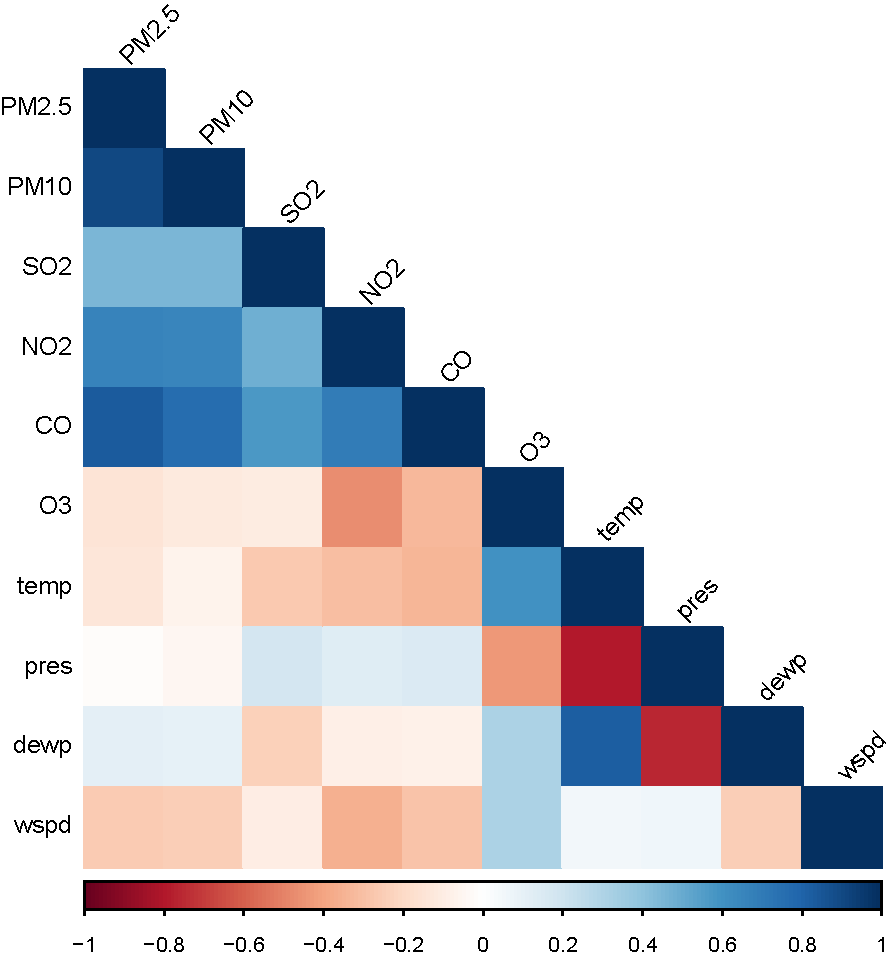
\includegraphics[width=0.8\textwidth]{resources/pdf/classic_correlation.pdf}
            \caption{Classic}
        \end{subfigure}
        \begin{subfigure}{0.49\textwidth}
            \centering
            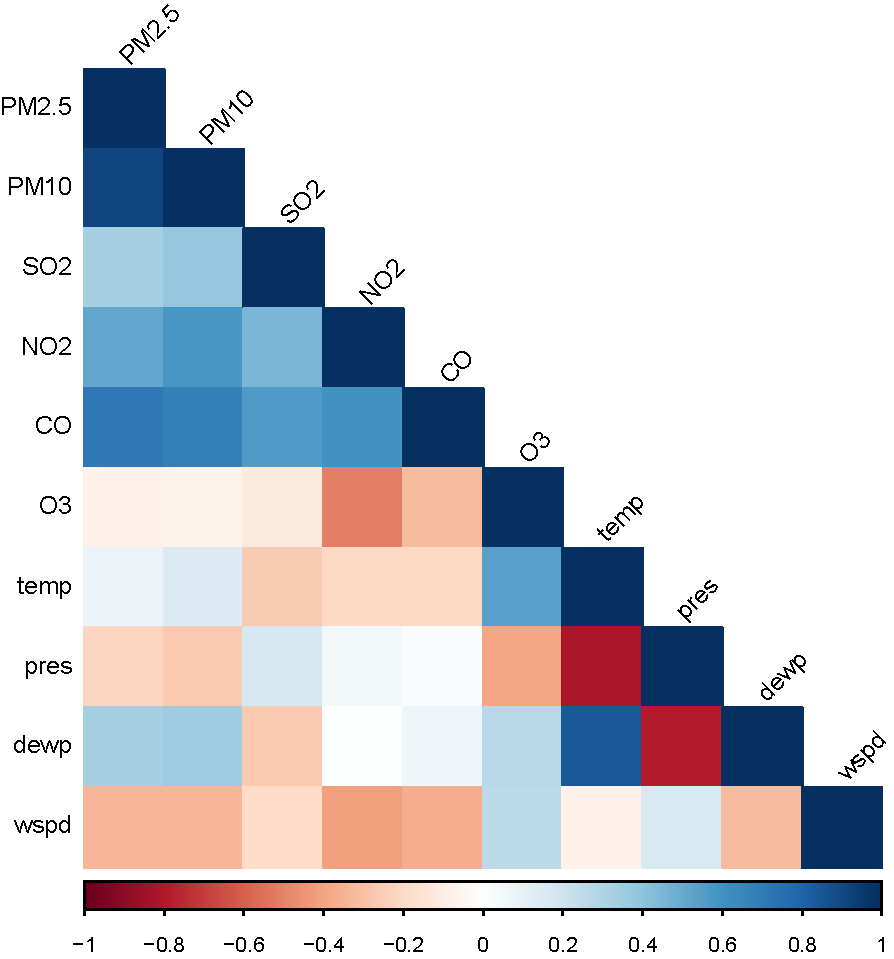
\includegraphics[width=0.8\textwidth]{resources/pdf/robust_correlation.pdf}
            \caption{Robust estimation}
        \end{subfigure}
        \noskipcaption{Graphical representation of the classic correlation matrix and a robust estimation of it.}
        \label{fig:robust_corrplot}
    \end{figure}
    
    As one can see in Figure \ref{fig:robust_corrplot}, both matrices are \emph{very} similar. This means that the outliers defined by the (reweighted) MCD estimator don't have much of an influence on the global correlation structure of the data set.
    
    \subsection{Graphic models}
    
    Using the \texttt{qgraph} function \cite{qgraph}, we have constructed the graphical models\footnote{All drawn edges have a weight of at least \num{e3}.} of the classical covariance matrix as well as an $L_1$-regularized estimation of it (cf. Figure \ref{fig:qgraphs}).
    
    \begin{figure}[h]
        \centering
        \begin{subfigure}{0.49\textwidth}
            \centering
            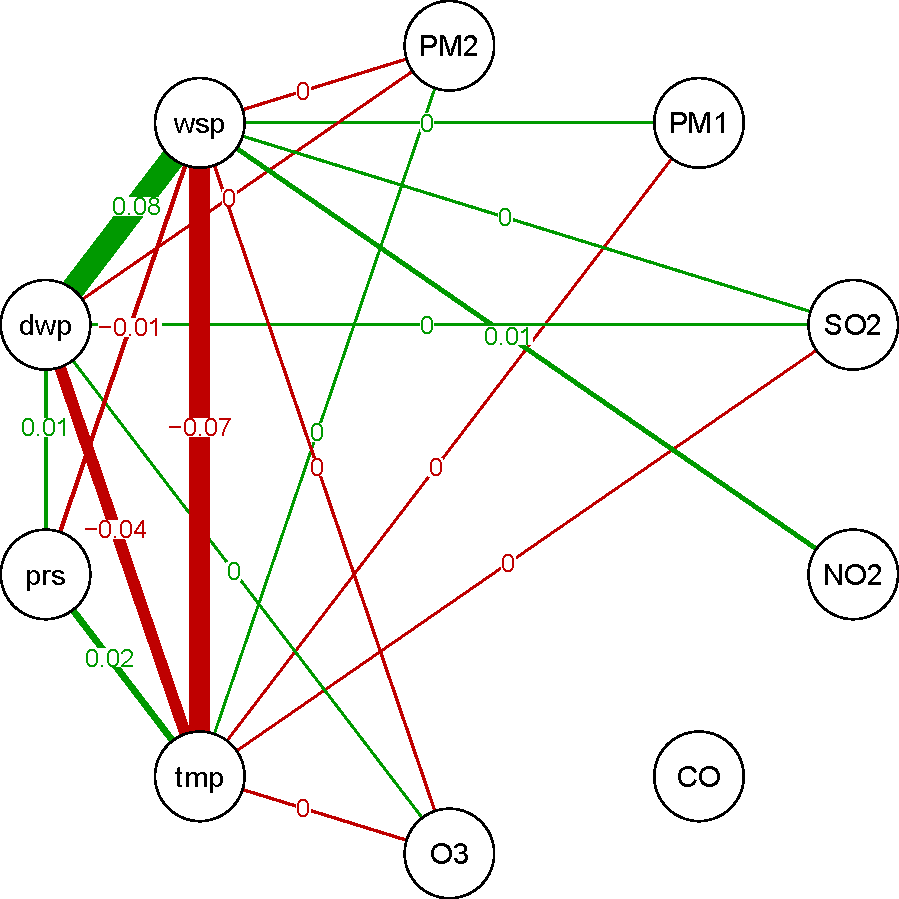
\includegraphics[width=0.8\textwidth]{resources/pdf/qgraph_classic_cov.pdf}
            \caption{Classic}
        \end{subfigure}
        \begin{subfigure}{0.49\textwidth}
            \centering
            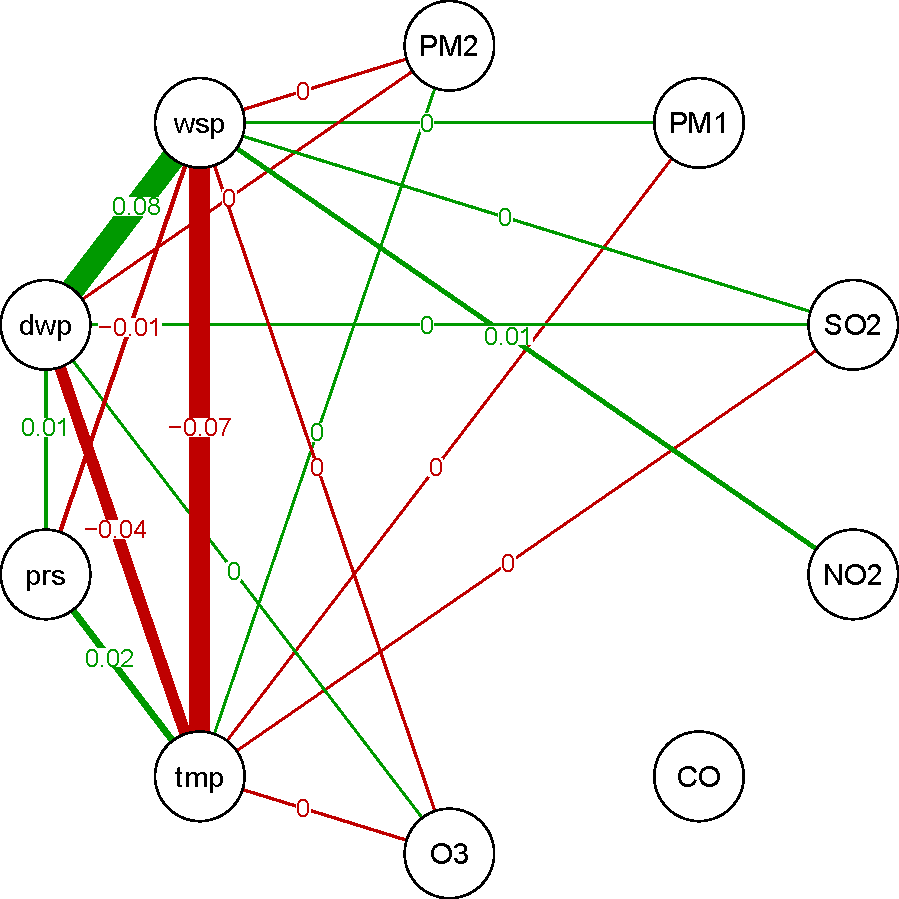
\includegraphics[width=0.8\textwidth]{resources/pdf/qgraph_l1_cov.pdf}
            \caption{$L_1$-regularized estimation ($\lambda = 0$)}
        \end{subfigure}
        \noskipcaption{Graphical models of the classic covariance matrix and an $L_1$-regularized estimation of it.}
        \label{fig:qgraphs}
    \end{figure}
    
    As one can see, the two models are \emph{exactly} the same. Indeed, the penalization parameter used is $\lambda = 0$, therefore the solution to the regularized maximum-likelihood optimization problem is the classic covariance matrix which explains why those models are the same. However, there is yet to explain why we have used such $\lambda$.
    
    There exists several proposals in the literature for selecting an appropriate value of $\lambda$ but, since it is the only one we have properly studied and applied, we decided to find $\lambda$ whose BIC measure is minimal. Therefore, we computed the BIC measure for several values of $\lambda$ and selected the one associated to the smallest BIC which appeared to be $0$ (cf. Figure \ref{fig:optimal_lambda}).
    
    In fact, this result is not surprising at all. The goal of the $L_1$-regularization is to make the concentration matrix (inverse of the covariance matrix), and therefore the graphical model, sparse(-er) but, as we can observe in the Figure \ref{fig:qgraphs}(a), the graphical model of the classic covariance matrix is \emph{already} quite sparse.
    
    \subsubsection*{Interpretation}
    
    Concerning the actual links drawn in the graphical models, we recognize some that we already had discussed in the project 1.
    
    For example, the relations between the atmospheric variables (temperature, pressure and dew point) we had drawn in the first project are also visible in the graphical models. We also recognize the dependencies between some pollutants and the temperature.
    
    There is also dependencies we hadn't noticed previously : the wind speed seems to have an influence over most other variables. Actually, this could explain why pollutant-to-pollutant relations are missing from the graphical models : if their concentrations are all dependent on the wind speed, pollutants should be conditionally independent (knowing the wind speed).
    
    \subsubsection*{Discussion}
    
    However, these graphical models are based on the multivariate normality assumption which is questionable for our dataset. Indeed, some variables such as temperature, dew point and pressure seem to follow normal distributions but all others don't, as discussed in the first project.

    But, this was considering the outliers as part of the dataset. If we don't, we see (cf. Figure \ref{fig:boxplots_outliers}) that PM2.5, PM10, \ce{NO2} and \ce{O3} are more likely to follow normal distributions. Therefore, the multivariate normality assumption isn't irrelevant, yet questionable.
    
    \section{Visualisation of the quantitative data in 2D}

    From the analysis detailed below, we notice that the principal component analysis seems to be far more informative by giving more interpretable results about the structure of the data while tSNE did not help us highlighting patterns in our data.

    \subsection{Principal component analysis} \label{PCA}

    In order to apply the principal component analysis, it has been chosen to use the correlation matrix instead of the covariance matrix\footnote{As a consequence, each time that we talk about variance in the subsections below, it's about the variance of the normalized data}. Indeed, the units and scales of our data were far to different to use them as is. This can be seen on Figure \ref{fig:covariance_plot}, which can be found in Appendix \ref{appendix_fig}.
    
    \begin{wrapfigure}{R}{0.5\textwidth}
	    \vspace{-1.5em}
	    \centering
	    \includegraphics[width=0.5\textwidth]{resources/pdf/pca_scree_plot.pdf}
	    \noskipcaption{Scree Plot of the eigenvalues of the correlation matrix.}
	    \label{fig:pca_scree_plot}
	    \vspace{-1em}
	\end{wrapfigure}

    Then, it has been chosen to use the classic estimation of the correlation matrix instead of the robust one. This can be justified a priori by the small differences between the robust estimation and the classic estimation of the correlation matrix. It has also been verified a posteriori that the PCA using the robust estimation gave quite similar results.

    The principal component analysis corresponds to finding the set of eigenvector and eigenvalues of the correlation matrix. In the basis of the eigenvectors, the data will thus seem completely uncorrelated. The ordering of the principal components (eigenvectors) is in decreasing order of the eigenvalues, such that the first component is the most explanatory of the correlation in our data. On the scree plot of Figure \ref{fig:pca_scree_plot}, we can see the percentage of the total variance (of the normalized data, as we use the correlation matrix) for each component. It can be computed that the first two principal component explain $68.49$\% of the total variance (of the normalized data).

    \begin{wrapfigure}{L}{0.45\textwidth}
        \vspace{-1em}
        \centering
        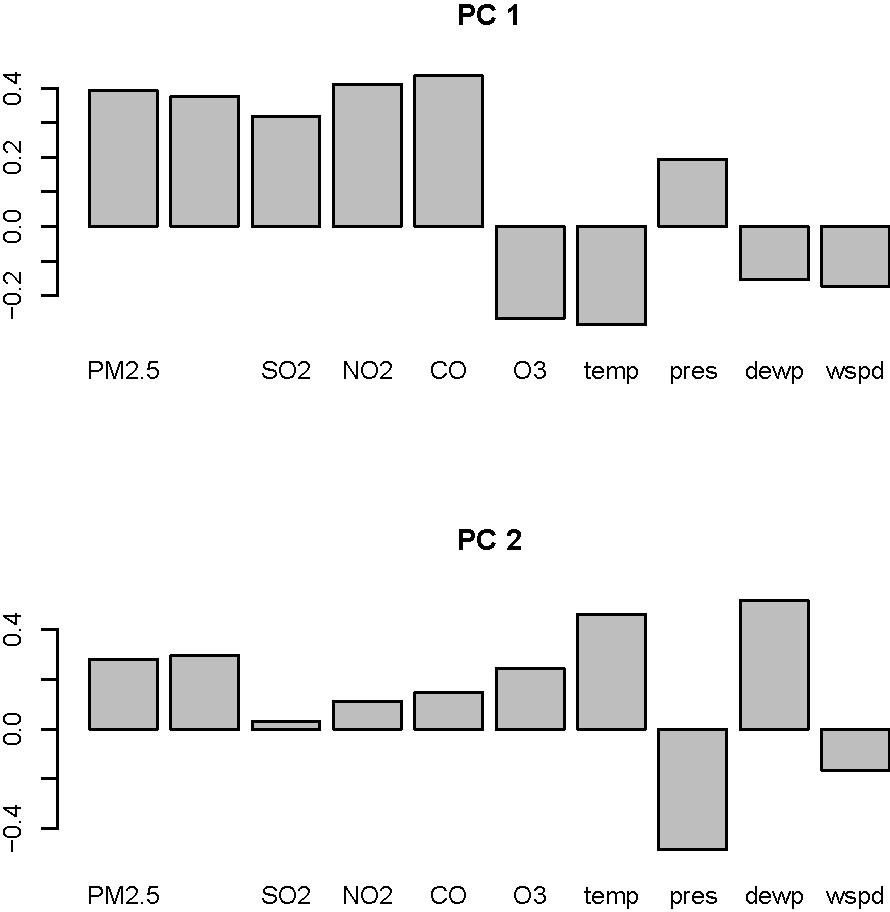
\includegraphics[width = 0.45\textwidth]{resources/pdf/pca_loadings.pdf}
        \caption{Loadings of the variables in the first two principal components}
        \label{fig:pca_loadings}
        \vspace{-1em}
    \end{wrapfigure}
    
    The loadings of the first two principal components can be used in order to get an interpretation of the meaning of these components. By looking at Figure \ref{fig:pca_loadings} it can been seen that the first component is mainly constituted of all the pollutants (only the O3 having a negative coefficient, accordingly to the correlation structure between the pollutants discussed in the first part of the project), while the second component is mainly composed of the atmospheric variable: the temperature, dew point, and pressure (only the pressure having a negative coefficient, being anti-correlated with the dew point and the pressure, accordingly to the correlation structure between these three variables spotted in the first part of the project). 

    This is quite interesting to see that $68\%$ of the variance of the data is contained in two independent components, the first corresponding roughly to the pollutants variable, and the second corresponding roughly to the atmospheric variables.

    The high eigenvalues of each of these two components tells us about the trend that have the data to vary according to these two independent components. The columns of the correlation plot of Figure \ref{fig:pca_variables_correlation} indicates the trend that have certain variables to vary together with the principal components, the first two columns gathering thus 68\% of this variation.

    On Figure \ref{fig:pca_explained_variability}, the squared correlation coefficients between each variable and each principal component have been plotted. Each element represents thus the part of variability of each variable explained by each principal component. We clearly see that every pollutant and atmospheric variable has its variability mainly explain by the two first principal components.
    
    \begin{figure}[h]
        \centering
        \begin{subfigure}{0.48\textwidth}
            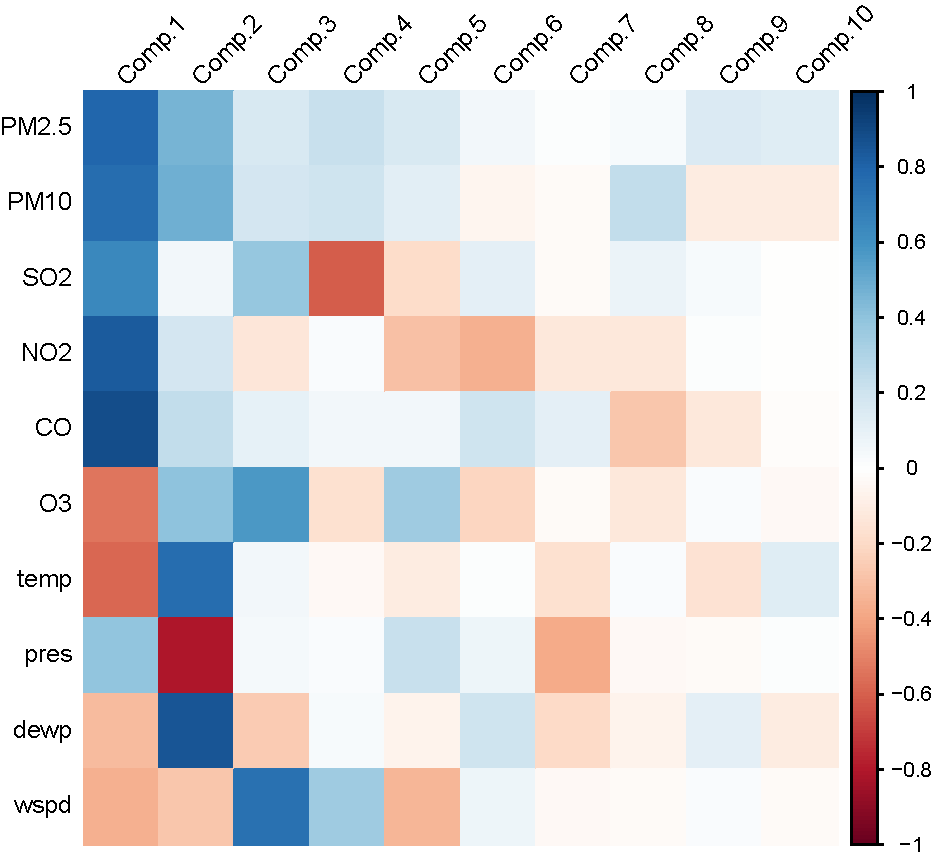
\includegraphics[width = \textwidth]{resources/pdf/pca_variables_correlation.pdf}
            \caption{Correlation between each variable and each principal component}
            \label{fig:pca_variables_correlation}
        \end{subfigure}
        \hspace{0.5em}
        \begin{subfigure}{0.48\textwidth}
            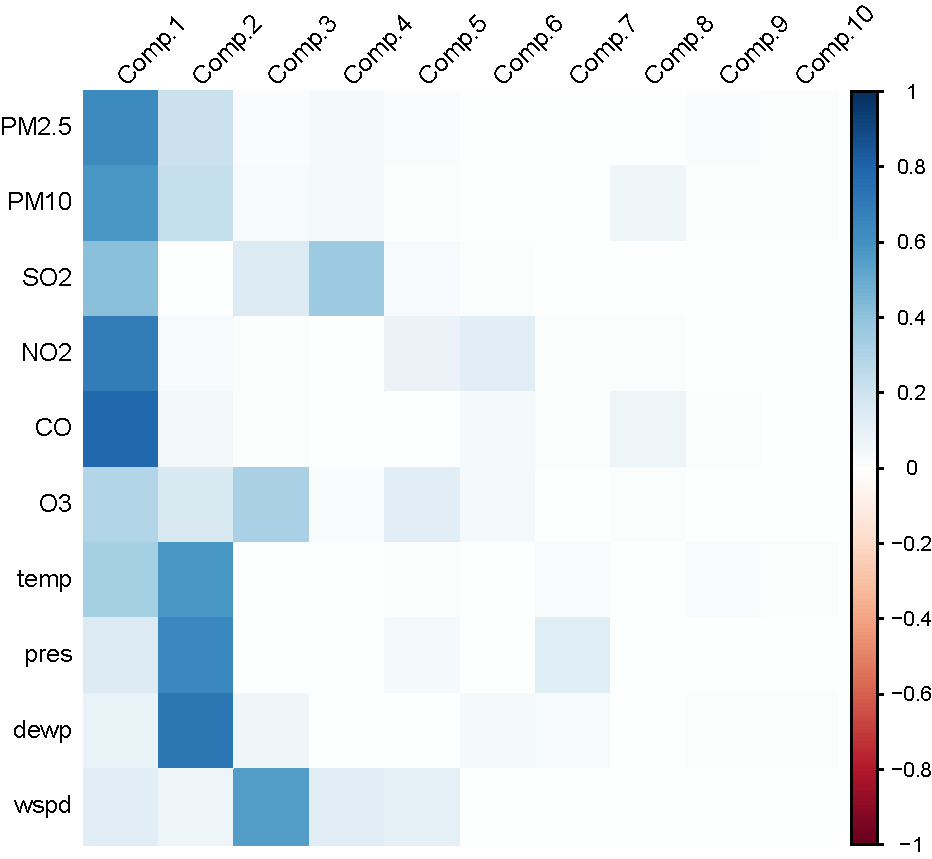
\includegraphics[width=\textwidth]{resources/pdf/pca_explained_variability.pdf}
            \caption{Squared correlation between each variable and each principal component}
            \label{fig:pca_explained_variability}
        \end{subfigure}
    \end{figure}

    All that is once again illustrated on the correlation circle of Figure \ref{fig:pca_correlation_circle}.

    \subsection{t-distributed stochastic neighbor embedding}
    \label{tSNE}

    The tSNE algorithm has been used in order to decrease the number of dimension to three or two. No clear pattern has be observed for any perplexity. 
    Moreover, our dataset having very few discrete data, no pattern has been detected by coloring the data points according to the rain, the moment of the day, the wind direction or the season of the year.

    It has also been tested to select the 20 most outlying observations according to the robust method, in order to see if the outliers belong to some clusters of data points. Although the outliers were indeed located in a certain number of clusters of the tSNE plot instead of being uniformly distributed, they were not located in very few cluster neither. 
    This could indicate that indeed some outliers are considered to be close in the quantitative data space, ending up in the same cluster in 2 dimensions. But that outliers could also come from very different location of the quantitative data space, ending up in different cluster in 2 dimensions.

    The result with of the tSNE algorithm can be seen on Figure \ref{fig:tSNE} for different perplexity values.
    
    \newpage
    
    \printbibliography
    
    \newpage
    \appendix
    
    \section{Figures} \label{appendix_fig}
    
    \begin{figure}[H]
        \centering
        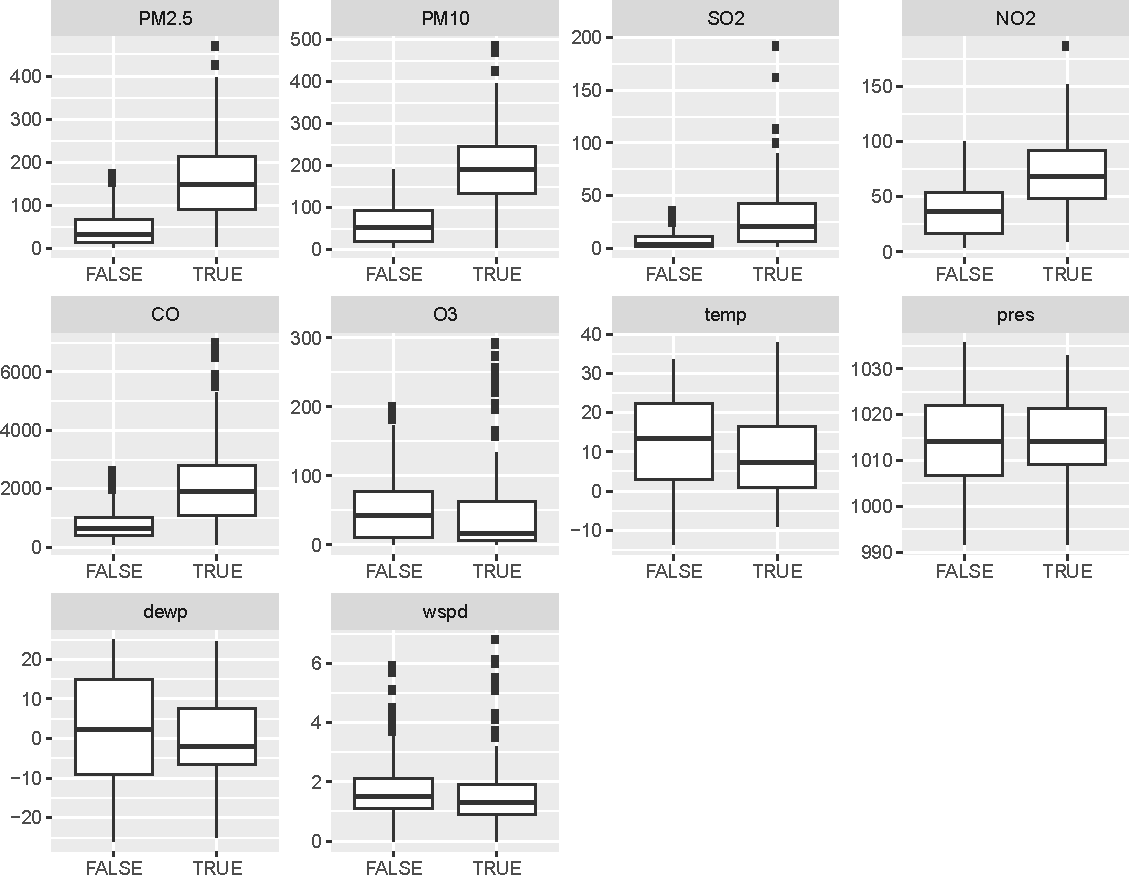
\includegraphics[width = \textwidth]{resources/pdf/boxplots_outliers.pdf}
        \caption{Boxplot of the quantitative variables for the non outlying observations (FALSE) and the robust outlying observations (TRUE).}
        \label{fig:boxplots_outliers}
    \end{figure}
    
    \subsubsection*{Detailed analysis of Figure \ref{fig:boxplots_outliers}}
    
    Concerning the pollutant concentrations\footnote{All the following rate computations can be found in the source code.}, we can clearly see that low \ce{O3} concentrations are present in both outlying and non outlying observations, while higher values are mainly met in the non outlying ones. Their quartiles look similar, the median of the outlying values being lower as both cases have a similar number of very low values. It should however be noticed that about \SI{7}{\percent} of outlying observations present concentration values above \SI{200}{\micro\gram\per\meter\cubed} while none of the non outlying ones does. These extreme concentration values do not seem to attract the outlying observations to extreme outliers, as can be seen from Table \ref{tab:6_extreme}.
    
    As far as CO is concerned, \SI{96}{\percent} of the non outlying concentrations are below \SI{2000}{\micro\gram\per\meter\cubed} while only roughly \SI{50}{\percent} of the outlying ones do. The other \SI{50}{\percent} are thus linked to CO concentrations above \SI{2000}{\micro\gram\per\meter\cubed} (with \SI{30}{\percent} of them being above the maximum non outlying CO concentration), while only \SI{4}{\percent} of the non outlying observations show values from \num{2000} to \num{2600} \si{\micro\gram\per\meter\cubed}, the maximum concentration observed. 
    
    For the \ce{NO2} concentrations, the median of the outlying observations is equal to \SI{68}{\micro\gram\per\meter\cubed}, while the one of the non outlying data points is \SI{36.5}{\micro\gram\per\meter\cubed} with \SI{12.5}{\percent} of these points being above the outlying median. About \SI{20}{\percent} of the outlying points have a concentration bigger than the maximum, achieved by only $1$ data point, of the non outlying ones.
    
    Concerning the \ce{SO2} concentrations, we can see that most of the non outlying observations are associated to very low values. Furthermore, about \SI{34}{\percent} of the outlying concentrations lie above the maximum concentration observed for the non outlying data, equal to \SI{36}{\micro\gram\per\meter\cubed}, again attained by only $1$ data point.
    
    Finally, a similar behavior can be noticed for both PM2.5 and PM10 concentrations, which will be analyzed in pair since they are positively correlated, as was shown in the first part of the project. As far as PM10 concentrations are concerned, none of the non outlying data points have a concentration value bigger than the median concentration of the outlying ones, equal to \SI{190.5}{\micro\gram\per\meter\cubed}. It thus also means that \SI{50}{\percent} of the outlying data points have concentrations above the maximum value observed in the non outlying data. Quite similar values are obtained for the PM2.5 concentrations: only \SI{2.5}{\percent} of non outlying points have values above the outlying median, and \SI{42}{\percent} of outlying points have values above the non outlying maximum PM2.5 concentration.
    
    \newpage
    
    \begin{figure}[H]
        \centering
        \includegraphics[width=0.66\textwidth]{resources/pdf/optimal_lambda.pdf}
        \caption{BIC measure with respect to the $\lambda$ penalization parameter.}
        \label{fig:optimal_lambda}
    \end{figure}
    
    \begin{figure}[H]
        \centering
        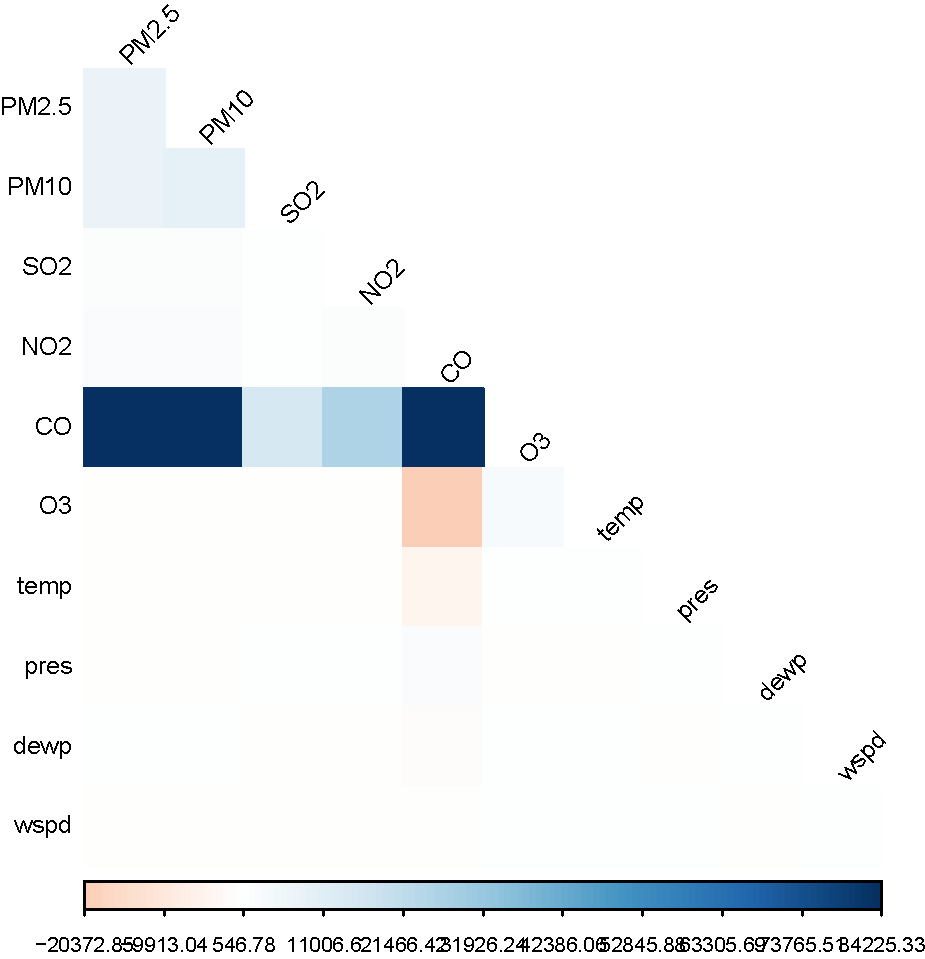
\includegraphics[width = 0.6 \textwidth]{resources/pdf/covariance_plot.pdf}
        \caption{Heat Map of the classic covariance matrix}
        \label{fig:covariance_plot}
    \end{figure}
        
    \begin{figure}[H]
        \centering
        \includegraphics[width=0.6 \textwidth]{resources/pdf/pca_correlation_circle.pdf}
        \caption{Correlation circle for the first two principal components}
        \label{fig:pca_correlation_circle}
    \end{figure}
    
    \begin{figure}[H]
        \centering
        \begin{subfigure}{0.49\textwidth}
            \includegraphics[width = \textwidth]{resources/pdf/tSNE_15.pdf}
            \caption{Perplexity of 15}
            \vspace{1em}
        \end{subfigure}
        \begin{subfigure}{0.49\textwidth}
            \includegraphics[width = \textwidth]{resources/pdf/tSNE_20.pdf}
            \caption{Perplexity of 20}
            \vspace{1em}
        \end{subfigure}
        \begin{subfigure}{0.49\textwidth}
            \includegraphics[width=\textwidth]{resources/pdf/tSNE_30.pdf}
            \caption{Perplexity of 30}
        \end{subfigure}
        \caption{tSNE of the quantitative data}
        \label{fig:tSNE}
    \end{figure}
    
    \section{Tables} \label{appendix_tab}
    \begin{table}[H]
        \centering
        \begin{tabular}{|c|c|c|c|c|c|c|c|c|c|c|}
            \hline 
            PM2.5 & PM10 & \ce{SO2} & \ce{NO2} & \ce{CO} & \ce{O3}  & temp & pres & dewp  & wspd & distance \\ \hline\hline
            199   & 292  & 113 & 115 & 6700 & 16  & -4.3 & 1025.0 & -11.3 & 2.4  & 279.3953 \\ \hline
            362   & 362  & 11  & 86  & 7000 & 8   & -0.3 & 1020.8 & -1.1  & 0.7  & 291.6911 \\ \hline
            74    & 379  & 3   & 50  & 300  & 64  & 26.3 & 1007.4 & -3.3  & 3.1  & 316.7818 \\ \hline
            256   & 321  & 162 & 108 & 5300 & 2   & 2.7  & 1025.8 & -2.8  & 0.5  & 460.6449 \\ \hline
            93    & 485  & 18  & 28  & 800  & 101 & 16.4 & 1017.3 & 3.4   & 1.2  & 560.9199 \\ \hline
            217   & 217  & 192 & 86  & 3800 & 4   & 2.1  & 1028.7 & -4.0  & 0.9  & 792.7060 \\ \hline
        \end{tabular}
        \caption{Values for the $6$ observations corresponding to the biggest robust Mahalanobis distances.}
        \label{tab:6_extreme}
    \end{table}
    
\end{document}
